\documentclass[11pt,letterpaper]{article}
\usepackage{geometry}%\geometry{left=1.5in,right=1.5in,}
\usepackage[utf8]{inputenc}
\usepackage{amsmath}
\usepackage{mathtools}
\usepackage{amsfonts}
\usepackage{amssymb}
\usepackage{graphicx}
\usepackage{caption}
\usepackage{subcaption}
\usepackage{enumerate}
\usepackage{listings}
\usepackage{color}
\usepackage{tikz}


% setup commands
\newcommand{\rank}{\mathrm{rank}}
\newcommand{\innerprod}[2]{\left\langle #1, #2 \right\rangle}
\newcommand{\abs}[1]{\left\lvert #1 \right\rvert}
\newcommand{\norm}[1]{\left\lVert #1 \right\rVert}
\newcommand{\Expect}[1]{{\rm I\kern-.3em E} \left[ #1 \right]}
\newcommand{\Var}[1]{\mathrm{Var} \left( #1 \right)}
\newcommand{\Cov}[1]{\mathrm{Cov} \left( #1 \right)}
\newcommand{\vect}[1]{\begin{bmatrix} #1 \end{bmatrix}}


% setup environment
\newenvironment{proof}{\paragraph{Proof:}}{\hfill$\square$}

\definecolor{codegreen}{RGB}{133,153,0}
\definecolor{codecyan}{RGB}{42,161,152}
\definecolor{codeblue}{RGB}{38,139,210}
\definecolor{base1}{RGB}{147,161,161} % comment
\definecolor{base3}{RGB}{253,246,227} % background
\definecolor{base00}{RGB}{101,123,131} % default code
\definecolor{base01}{RGB}{88,101,117} % optional emphasized content
\lstdefinestyle{codestyle}{
	backgroundcolor=\color{base3},   
	basicstyle=\footnotesize\color{base00},
	numberstyle=\tiny\color{base00},
	commentstyle=\color{base1},
	keywordstyle=\bfseries\color{codegreen},
	stringstyle=\color{codecyan},
	%identifierstyle=\color{codeblue},
	breakatwhitespace=false,         
	breaklines=true,                 
	captionpos=b,                    
	keepspaces=true,                 
	numbers=left,                    
	numbersep=5pt,                  
	showspaces=false,                
	showstringspaces=false,
	showtabs=false,                  
	tabsize=4
}

% information
\author{Khoi-Nguyen Mac}
\title{ECE551 - Project Proposal \\ RGB-D Object Recognition using Multimodal Deep Learning}

\begin{document}
\maketitle
	
\section{Motivation}
Object recognition is a popular problem that draw much attention from different researches. Since images are actually two dimensional signals, this project fits in the scope of Digital Signal Processing II course. Furthermore, convolutional neural networks (CNNs) in the recent years are proved to be highly efficient for object recognition and thus have been explored by large companies such as Google, IBM, Facebook, etc. In the sense of signal processing, the convolutional layers of such networks play the role of filter banks, where input signals are images and outputs are their representation in probability domain, corresponding to some sets of categories. Another motivation for this project is the popularity of depth cameras, making it easy to produce depth images. The availability of such information can enrich the input data and thus can increase the recognition accuracy.

\section{Project Description}
The goal of this project is to implement a deep learning system based on CNN architecture that can receive color and depth images from an object and predict which category such object belongs to. As the system has to work with two different channels of data, there has to be some fusion mechanism to combine the features. 

In this project, I propose to explore the technique of the 2015 paper \textit{Multimodal Deep Learning for Robust RGB-D Object Recognition} \cite{DBLP:journals/corr/EitelSSRB15}, by Eitel et al. As illustrated in Figure \ref{fig:eitel_archi}, their network consists of two channels, corresponding to color and depth images, whose architectures are based on AlexNet. There are fully connected layers at the end of the network to fuse features extracted from the channels. Since AlexNet is used, the network is initialized with AlexNet weights, which are pretrained from ImageNet dataset. However, AlexNet is only created for recognizing objects with color images, therefore the depth maps is converted to color domain so that it can work with the architecture.

\begin{figure}
	\centering
	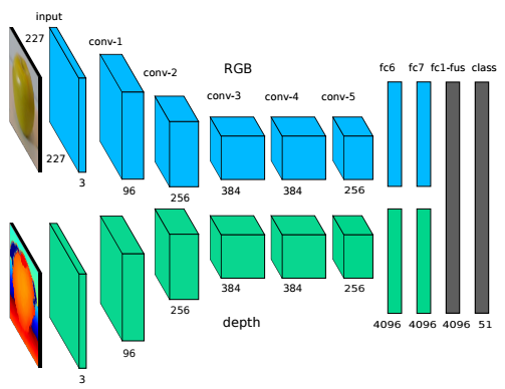
\includegraphics{Picture1}
	\caption{Convolutional Neural Networks with multichannel architecture proposed by Eitel et al \cite{DBLP:journals/corr/EitelSSRB15}.}
	\label{fig:eitel_archi}
\end{figure}

It can be seen that the fusion technique is mainly comprised in the fully connected layers at the end of the network. Although this approach can improve recognition accuracy from single channel models, the method is straightforward. Therefore, I propose to implement a more complicated fusion technique that can fuse the layers throughout the whole network. Considering the first convolutional layer, the technique's concept is showed in Figure \ref{fig:my_archi}. Let $(W_1^C, b_1^C)$ and $(W_1^D, b_1^D)$ be trained parameters (weights and biases) of the first layer, where $C$ and $D$ denote color and depth channel, respectively. The output features, $conv_1^C$ and $conv_1^D$, are fused together with fusion operator to make $x^F$. This $x^F$ serves as the input for the first fusion layer, whose parameters $(W_1^F, b_1^F)$ are to be trained. The output $fus_1$ is decomposed by a decomposition operator, which can be seen as the adjoint operator of fusion, and fed to the next layers. This proposed technique will be tested against the method in \cite{DBLP:journals/corr/EitelSSRB15}, which is implemented as the baseline.

\begin{figure}
	\centering
	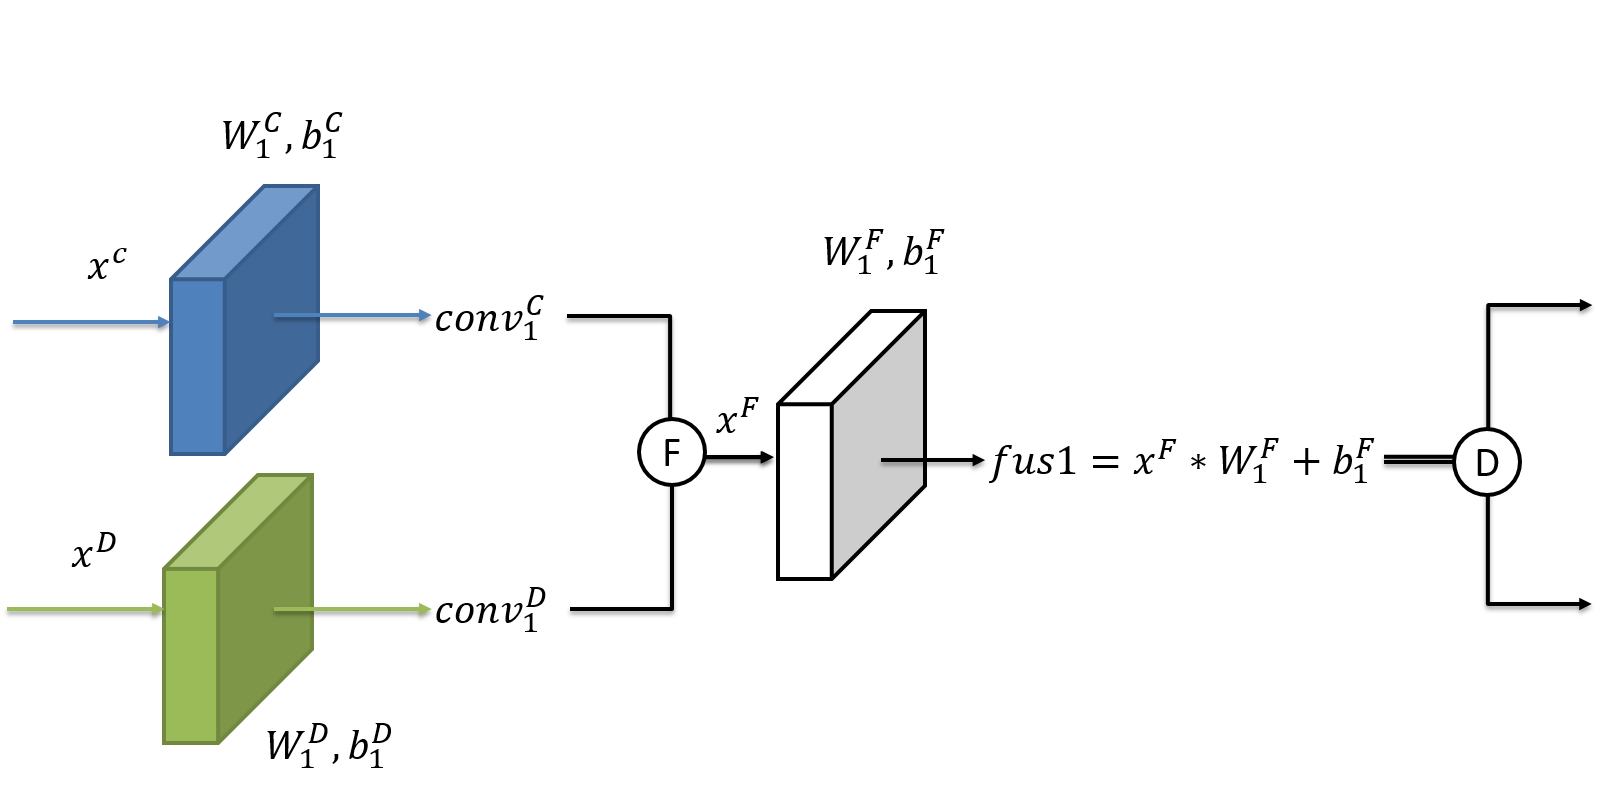
\includegraphics[width=\textwidth]{Picture2}
	\caption{Proposed fusion method, in the scope of one convolutional layer.}
	\label{fig:my_archi}
\end{figure}

\section{Resources}
I propose to use Washington's RGB-D object dataset to train and validate results as this is the dataset used in \cite{DBLP:journals/corr/EitelSSRB15} and also is a benchmark in other papers about object recognition. The system is implemented using Python and TensorFlow framework. Although this is a new framework, it is reliable since it is used in several recent researches in machine learning field and is supported by Google. No outside code other than pretrained weights from AlexNet will be used.

\bibliographystyle{plain}
\bibliography{ref}
\end{document}